
\begin{frame}[noframenumbering]{Theme alternative: Faculty of App. Computer Science}
    \hspace{1cm}\includegraphics[height=.7\paperheight]{./../latex-beamer-template/rendered-preview-pictures/FAICompilation.png}
\end{frame}

\note[enumerate]{
    \item Template does also do "Faculty of Applied Computer Science" presentations out of the box
    \item Alternate styles (e.g. title slide) available
}

\begin{frame}[noframenumbering]{Backup-Solution Problem 1}
    \hspace{2cm}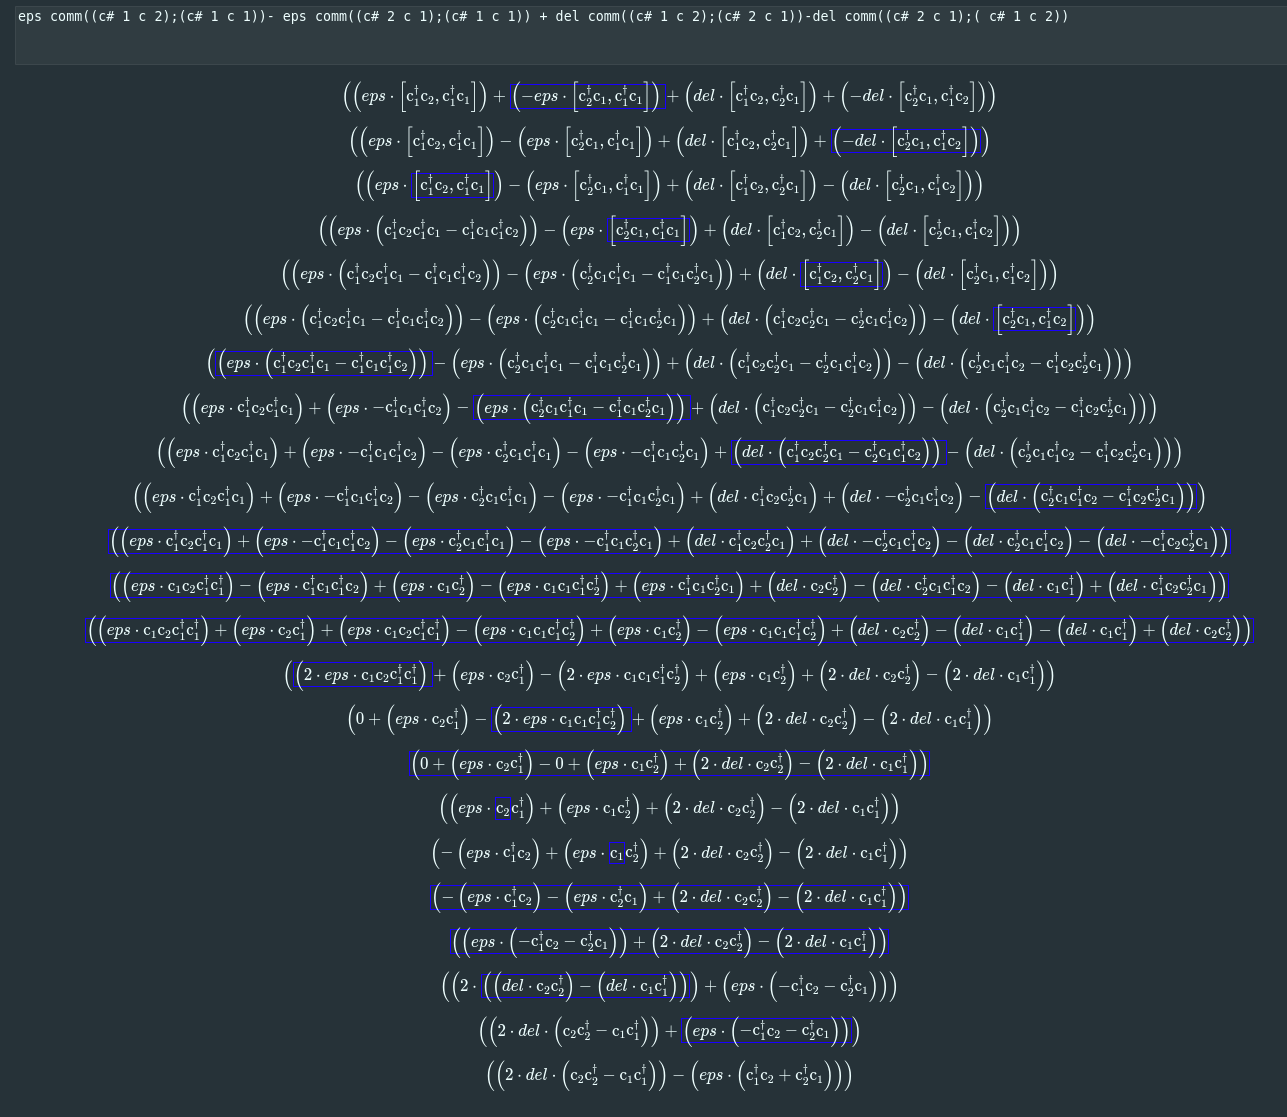
\includegraphics[height=.72\paperheight]{./math-manipulator-calculations/fkp_page_15_backup_solution.png}
\end{frame}

\begin{frame}[noframenumbering]{Backup-Solution Problem 2}
    \hspace{0.6cm}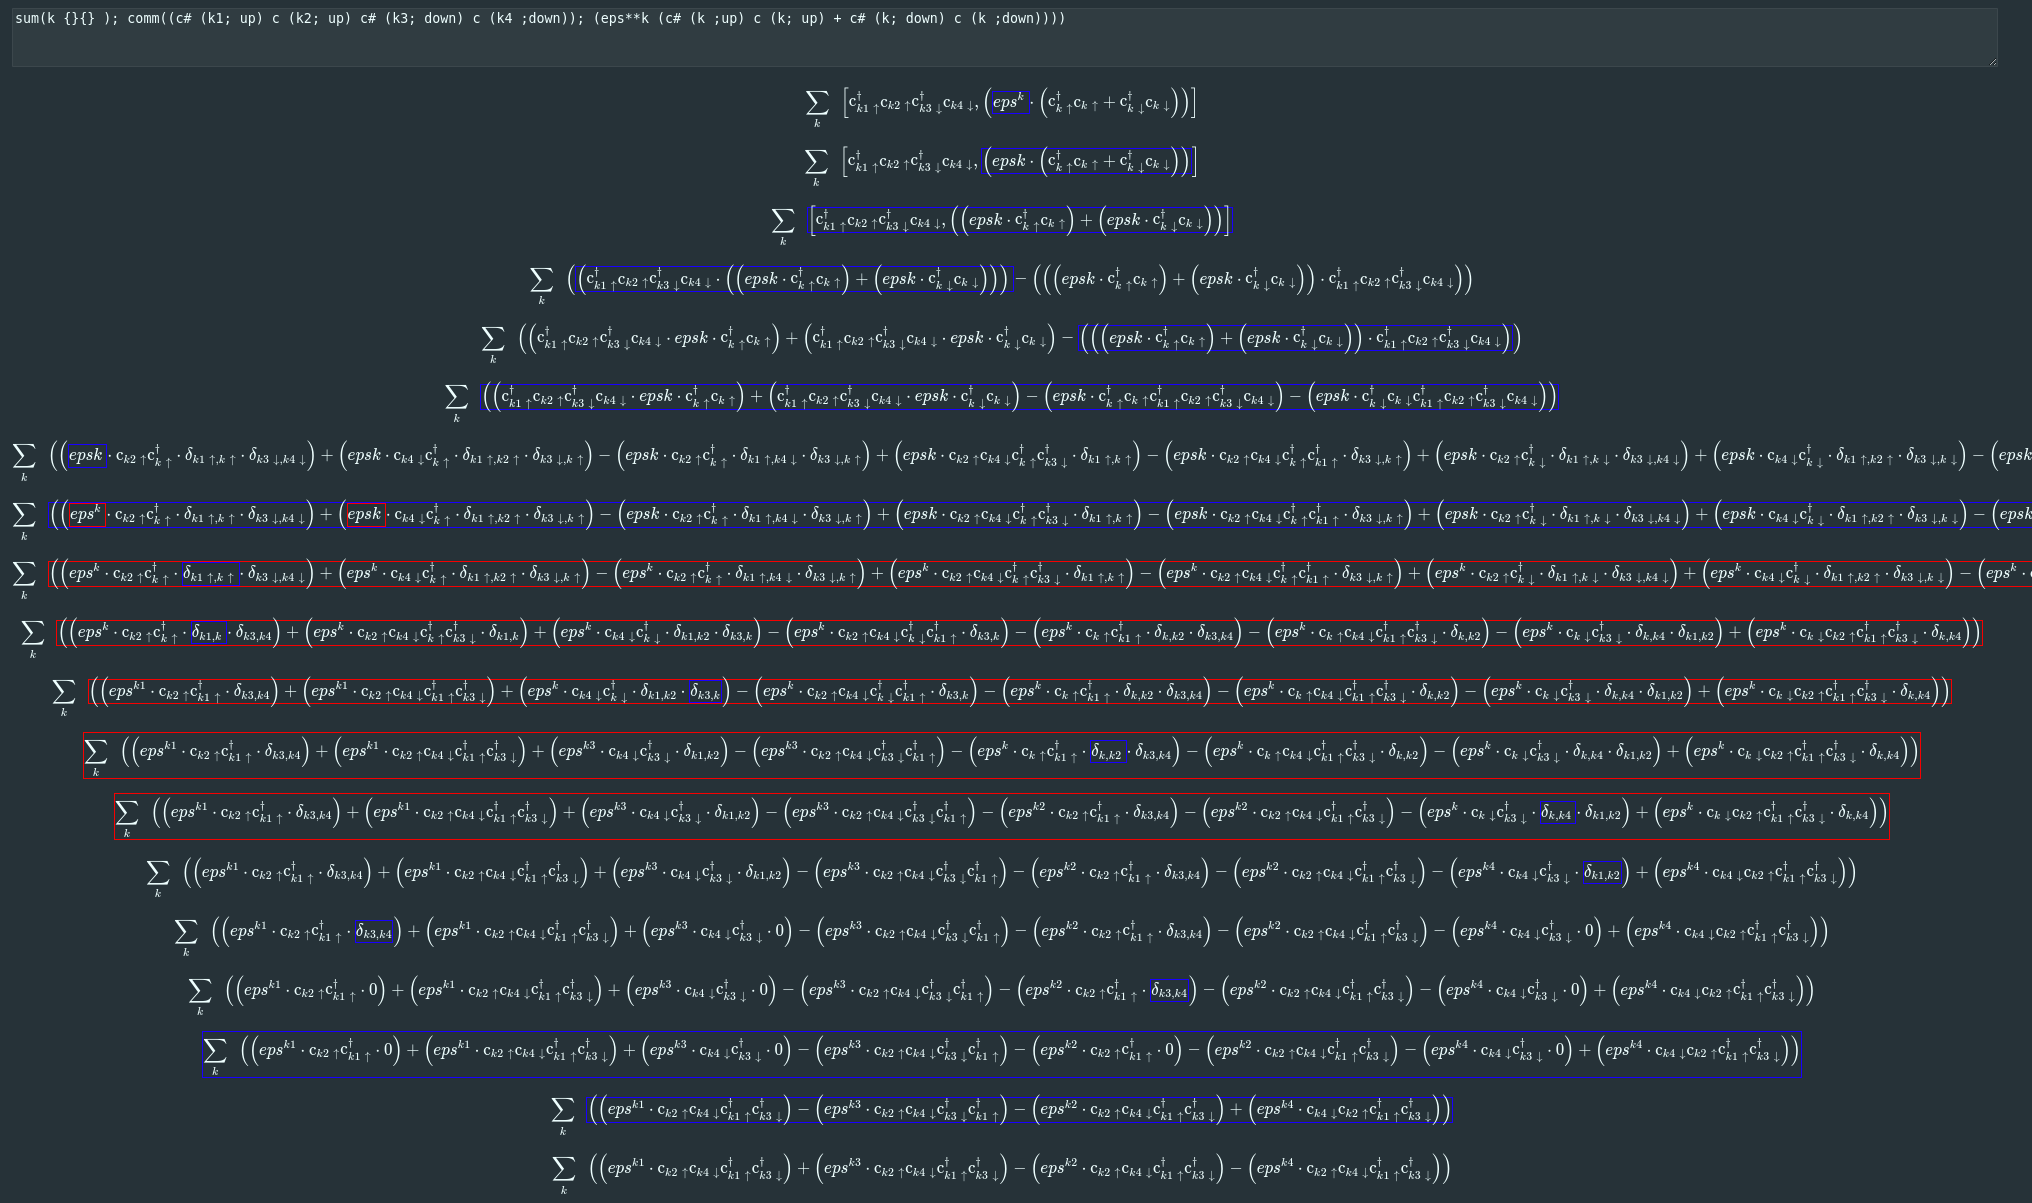
\includegraphics[height=.72\paperheight]{./math-manipulator-calculations/fkp_page_33_backup_solution.png}
\end{frame}

\begin{frame}[noframenumbering, t]{Backup: Simplification V-Parts}
    \vspace{-0.2cm}
    \begin{minipage}[t]{0.6\textwidth}
        \vspace{0pt}
        \hspace{-2em}
        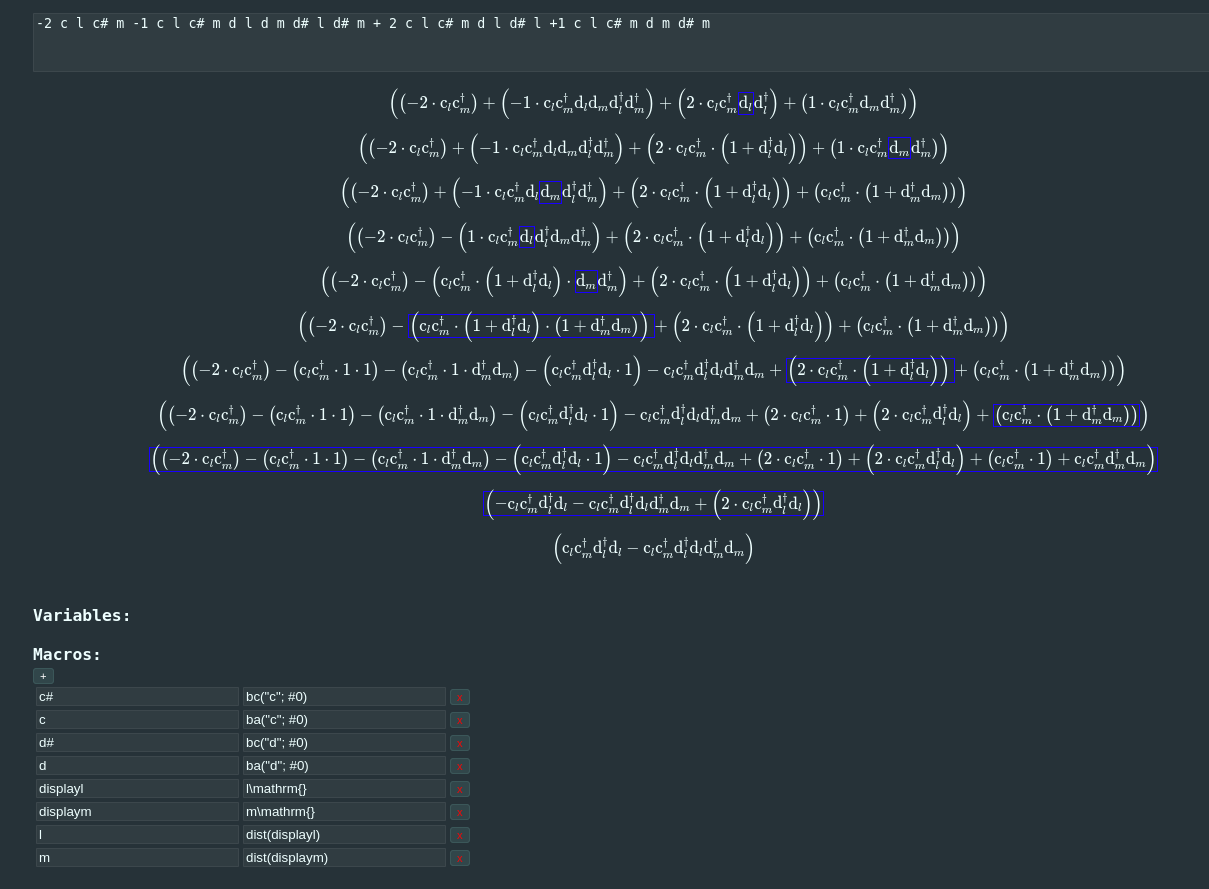
\includegraphics[width=.5\paperwidth]{./math-manipulator-calculations/simplification_cparts_backup_solution.png}
    \end{minipage}%
    \begin{minipage}[t]{0.6\textwidth}
        \vspace{0pt}
        \hspace{-3em}
        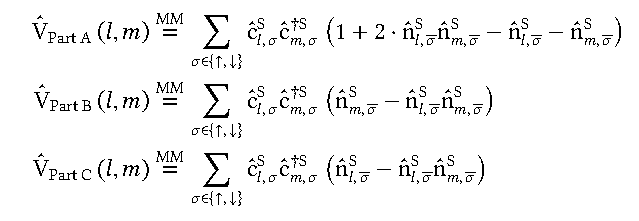
\includegraphics[width=.41\paperwidth]{./math-manipulator-calculations/simplification_cparts.pdf}
    \end{minipage}
\end{frame}

\note[enumerate]{
    \item Better optimization was found, rewriting in number operators DOES save on terms (however only for B and C, A still same number of terms and computational requirement, even if it looks nicer)
    \item Doesn't help at all with computing more efficiently, so python script still exceptinally usefull
    \item Wouldn't have come so far, if simple "brute-force" solution wasn't done in the first place
}
